\chapter{研究方法}
\section{問題定義}
使用深度學習在歌聲分離領域上,本論文採取監督式學習訓練,取音樂訊號的頻譜(spectrogram)後,對其做值域轉換成為模型訓練使用的特徵,模型的輸出應為主唱(vocals stem)與伴奏(accompaniment stem)的頻譜,現在主流的架構建立於 U-Net~\cite{ronneberger2015u,jansson2017singing,hennequin2020spleeter,defossez2019music} 之上,憑藉其在圖像分割領域卓越的表現,期許在頻譜圖也能有所突破。對於 U-Net 的輸出,是否能經過簡單的處理就能提高其預測質量也是一個值得探討的問題。另外,在實際部屬 U-Net 模型時有個不可漠視的問題,其龐大的架構不適合在行動裝置上與晶片上搭載,會面臨模型預測時間長與裝置記憶體不足的問題。本論文的研究建立在現有的 U-Net 模型架構上進行分析與改良,主要有:
\begin{itemize}
	\item[1.] 基於 ratio mask filter 與 Wiener filter 理論,善加利用現有的 U-Net 模型之預測頻譜圖,以提升輸出質量。
	\item[2.] 研究不同的 U-Net 架構,本篇會著重在注意力模型 attention gate 與 self-attention 的基礎上做延伸,設計一新的 U-Net 模型,並測試對於分離歌聲的效果。
	\item[3.] 基於先前頻譜刪減(spectral subtraction)~\cite{boll1979suppression} 的研究,探討其問題與設法提升其效果。
	\item[4.] U-Net 模型壓縮實驗,使用模型剪枝(model pruning)與模型量化(model quantization)來達成。
\end{itemize}

\section{實驗環境}
\begin{itemize}
    \item Server
    \subitem CPU:{\bf Intel(R) Xeon(R) Silver 4116 @ 2.10GHz}
    \subitem RAM:{\bf 314 GB}
    \subitem GPU:{\bf NVIDIA Quadro GV100 and NVIDIA TITAN RTX}
    \item Edge device
    \subitem Model name:{\bf Raspberry Pi 4 Model B}
    \subitem CPU:{\bf Quad core Cortex-A72 (ARM v8) 64-bit SoC @ 1.5GHz}
    \subitem RAM:{\bf 4GB}
    \subitem GPU:{\bf None}
\end{itemize}


\section{評量指標}
Vincent~\cite{vincent2006performance} 提出的指標評量以比較「原始聲音」與「預測聲音」的差距與量化,在本論文中,探討的是「原始音軌」與「U-Net 模型預測的音軌」。本篇使用的是 Python 套件 Museval~\cite{stoter2018museval}\footnote{\url{https://github.com/sigsep/sigsep-mus-eval}},一個以前述指標包裝而成的套件,由 SegSep\footnote{\url{https://sigsep.github.io/}} 團隊維護而成,並在 2018 signal separation evaluation campaign~\cite{stoter20182018} 中所採取,此領域的研究也以此做為評估指標,這些都代表著其重要程度,適合被本論文所採取。Museval 使用 Musdb18~\cite{rafii2017musdb18,musdb18} 的測試集做 Vincent 定義的指標,以該資料集中每一首歌每秒為單位,比較「原始聲音」與「預測聲音」的差距,並以 json 格式儲存後以便上傳至比賽單位,最後做整體評估~\cite{stoter20182018}時,在每首歌中的評量裡取其中位數作為該歌曲的得分,在該資料集中取其中位數作為該資料集的得分。Vincent 定義分離的訊號是由 4 個元素組成,等式如下:
\begin{equation*}
    \widehat{s_j}=s_\textup{target}+e_\textup{interf}+e_\textup{noise}+e_\textup{artif}
\end{equation*}
其中:
\begin{itemize}
    \item $s_\textup{target}$:目標來源的訊號(為目標音軌的原始聲音)
    \item $e_\textup{interf}$:表示其他來源訊號的干擾(為其他音軌參雜而導致的噪音)
    \item $e_\textup{noise}$:表示訊號中的雜訊
    \item $e_\textup{artif}$:額外產生的干擾(為 U-Net 在預測過程中產生的噪音)
\end{itemize}
Vincent 依照上面定義設計了 SDR、SIR 與 SAR 指標:
\begin{itemize}
    \item Source-to-Distortion Ratio(SDR):此指標為評量分離結果的總失真程度,當 SDR 值越高時,代表分離結果與實際訊號的總失真越低;反之,當 SDR 值越低時,代表總失真越高。
        \begin{equation*}
        SDR:=10\log_{10}\frac{\|s_\textup{target}\|^2}{\|e_\textup{interf}+e_\textup{noise}+e_\textup{artif}\|^2}
        \end{equation*}
    \item Source-to-Interferences Ratio(SIR):此指標為評量分離結果受其他來源干擾的程度,當 SIR 值越高時,代表分離結果受其他來源干擾越低;反之,當 SIR 值越低時,代表受其他來源干擾越高。
        \begin{equation*}
        SIR:=10\log_{10}\frac{\|s_\textup{target}\|^2}{\|e_\textup{interf}\|^2}
        \end{equation*}
    \item Sources-to-Artifacts Ratio(SAR):此指標評估模型預測時額外產生的干擾程度,當 SAR 值越高時,代表在分離結果中,額外產生的干擾程度越低;反之,當 SAR 值越低時,代表額外產生的干擾程度越高。
        \begin{equation*}
        SAR:=10\log_{10}\frac{\|s_\textup{target}+e_\textup{interf}+e_\textup{noise}\|^2}{\|e_\textup{artif}\|^2}
        \end{equation*}
\end{itemize}
基於上面指標的描述,也根據這篇問答\footnote{\href{https://dsp.stackexchange.com/questions/9610/snr-calculation-in-audio-reconstruction-and-what-is-an-acceptable-value}{Stackexchange Q\&A}},本輪文的研究可泛用在KTV產業界中,主要以提升伴奏質量為優先。可以注意的是,在必要的妥協下,可以捨去 SIR (伴奏中可以出現些許的主唱),專注提升 SAR (減少 U-Net 模型賦予的噪音),使 short-time-fourier-transform 的 window 越大可讓 SIR 提升而讓 SAR 下降。

\section{實驗設計與方法}
下文裡實驗中的模型,只使用 Musdb18 中的資料以訓練,以本文的實驗基準 U-Net 來說,使用所有的資料集進行完整訓練,大約需要14天,但若只使用 Musdb18 進行訓練,只需2天即可,另外 Demucs~\cite{defossez2019music} 的研究中,也有只使用 Musdb18 作為訓練的實驗,綜觀考量之下,本論文採取此做法以節省時間,但在最後挑出的最好模型,仍會進行一次完整資料集的訓練,確認模型效能。

\subsection{神經模型訓練設定}
\begin{itemize}
    \item Feature extraction
    \subitem Sample frequency:44.1 kHz
    \subitem Frame size:4096
    \subitem Step size:1024
    \subitem Feature (neural net input):$\log_e{1+\vert X\vert} $, $\vert X\vert$ stands magnitude of signal
    \subitem Cropping: Frequency bin(F)to 2048 and frame size(T) to 216
    \item Neural net training (PyTorch environment)
    \subitem Epoch:200
    \subitem Batch size:6
    \subitem Optimizer:Adam~\cite{kingma2014adam}
    \subitem Learning rate:0.0001
    \subitem Loss:smooth L1 loss\footnote{\url{https://pytorch.org/docs/stable/generated/torch.nn.SmoothL1Loss.html}}
    \subitem LR scheduler:reduce lr on plateau\footnote{\url{https://pytorch.org/docs/stable/optim.html}}
\end{itemize}
這邊採取的 smooth L1 loss 函數可以視為平滑版的 L1 loss 函數(圖\ref{xLxLoss1})。當預測值 $f(x_i)$ 與對應的正確值 $y_i$ 差異較小時(絕對差小於1),smooth L1 loss 函數其實是使用了 L2 Loss,使梯度不會太大;在差異大時,採取類 L1 loss 函數的方法,梯度穩定,不導致梯度爆炸。通常 smooth L1 loss 函數應用在大多數問題,亦在本論文的實驗中。

\begin{equation*}
    loss(x,y)=\frac{1}{n}\sum_{i=1}^{n}\left\{\begin{matrix}
        0.5 \times (y_i-f(x_i))^2,& \textup{if}\ \vert y_i-f(x_i)\vert < 1\\ 
        \vert y_i-f(x_i)\vert -0.5,& \textup{otherwise}
    \end{matrix}\right.
\end{equation*}

\begin{figure}[htbp]
    \hfil
    \begin{minipage}[t]{0.6\textwidth}
        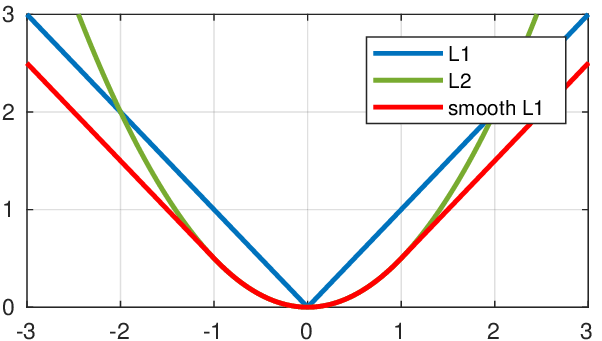
\includegraphics[width=\textwidth]{./figures/chapter04_experiment/xLxLoss1.png}
        \caption {Loss 函數比較圖}
        \label{xLxLoss1}
    \end{minipage}
    \hfil
\end{figure}

\subsection{濾波實驗}
本節說明濾波實驗的緣由。基於既有已訓練的 U-Net baseline 模型,採取適合的後處理也很重要,本論文主要探討 ratio mask filter 與 Wiener filter 作為後處理對模型預測的增幅。Python 套件 norbert~\cite{liutkus2019sigsep}\footnote{\url{https://github.com/sigsep/norbert}} 將此包裝,並在本實驗過程中使用。既有 U-Net 的輸出為頻譜域,要將其轉換為時間域,過去的方法是直接與混音軌的相位合併,再使用 iSTFT 轉回(圖\ref{Filter1}),本論文將 U-Net 的輸出頻譜轉換為一個濾波器,再對混音軌的 STFT 域做過濾(圖\ref{Filter2}),並在下章比對其效能。

\begin{figure}[htbp]
    \hfil
    \begin{minipage}[t]{0.8\textwidth}
        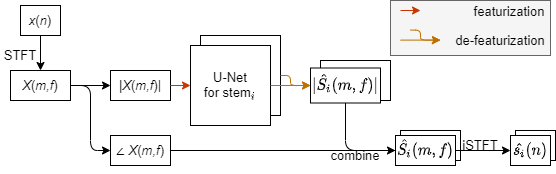
\includegraphics[width=\textwidth]{./figures/chapter04_experiment/Filter1.png}
        \caption {原始轉換方法}
        \label{Filter1}
    \end{minipage}
    \hfil
\end{figure}

\begin{figure}[htbp]
    \hfil
    \begin{minipage}[t]{0.8\textwidth}
        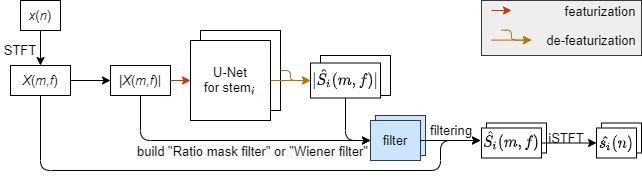
\includegraphics[width=\textwidth]{./figures/chapter04_experiment/Filter2.png}
        \caption {本論文轉換方法}
        \label{Filter2}
    \end{minipage}
    \hfil
\end{figure}

\subsubsection{頻譜刪減法}
在先前的實驗中,成功的將下式套用在歌聲分離領域:
\begin{equation}
	\|X(\omega)\|^2=\left\{\begin{matrix}\|Y(\omega)\|^2-\alpha\cdot\|R(\omega)\|^2,\ \ \ if\ \ \|Y(\omega)\|^2-\alpha\cdot\|R(\omega)\|^2 > 0
\\ 
0,\ otherwise
\end{matrix}\right.
\end{equation}
其中 $\alpha$ 控制刪減的幅度,在 U-Net 預測出主唱聲與伴奏頻譜以經頗為優越的情況下,以此演算法得到更佳的輸出,經數據證明,在 $\alpha=0.2$ 的時候,其效果有些許地增幅,數據會與本次實驗放在下一章做比較。
因此,將頻譜刪減法套用於歌聲分離領域是可行的,本論文將會著重在各個頻譜中,控制每個不同 frequency bin 在不同刪減的幅度 $\alpha$ 的情況下,是否可以得到更好的效果,本論文會以兩種方式對此探討。

第一種方式,最直覺的作法就是對"每個" frequency bin $f$ 窮舉所有的 $\alpha_f$,在一個給定的資料集下,找到對應最好的刪減幅度,但這會面臨到四個問題:frequency bin 太多(一個模型輸出的頻譜有 2048 個 frequency bin)、 $0\leq\alpha_f\leq1$ 之間的實數要如何枚舉、資料集大小的界定、窮舉所有 $\alpha_f$ 的可行性。在時間與現有機器的妥協下,本論文實驗以一種較為單純可行的設定進行:

\begin{itemize}
    \item[1.] frequency bin 太多(頻譜有 2048 個 frequency bin)
        \subitem 以 256 個 frequency bin 化為一個頻帶 $b$(frequency subband),可劃分為 8 個頻帶
    \item[2.] 枚舉 $0\leq\alpha_b\leq1$ 之間作為刪減幅度的可能
        \subitem 以一個 0.1 的躍幅(hop size)取值,對每個頻帶 $b$(第一點提及),一共考慮 11 種刪減幅度的可能
    \item[3.] 資料集大小的界定
        \subitem 以 Musdb18 的一個 7 秒資料集作為參考,其中有 144 首音樂,主要考慮其資料集的多樣性而非完整的一首歌
    \item[4.] 窮舉所有 $\alpha_b$ 的可行性
        \subitem 就算已經將實驗化簡至此,對模型輸出的一組頻譜,要窮舉出所有的幅度也還需要 $11^8$ 的計算量,對整個資料集所有歌的計算量就為 $11^8\times144$,每個計算量又要將 Museval 的評估時間納入,這幾乎難以實現。因此,本論文以一種基礎為假設,每個頻帶之間是獨立的,在計算一個頻帶的刪減幅度 $\alpha_b$ 時,其餘頻帶保持原始 U-Net 的輸出,命名為「區域頻帶最佳解」(Band’s Optimum Ratio),請參照圖\ref{Bands_Optimum_Ratio}、圖\ref{Bands_Optimum_Ratio2}與圖\ref{Local_Bands_Optimal3}的說明會更好理解,如此一來在整個資料集的計算量,可大幅降低至 $11\times8$ ,這種折衷的辦法是否能達到效果,會在下章仔細的探討與分析。
\end{itemize}
\begin{figure}[htbp]
    \hfil
    \begin{minipage}[t]{0.65\textwidth}
        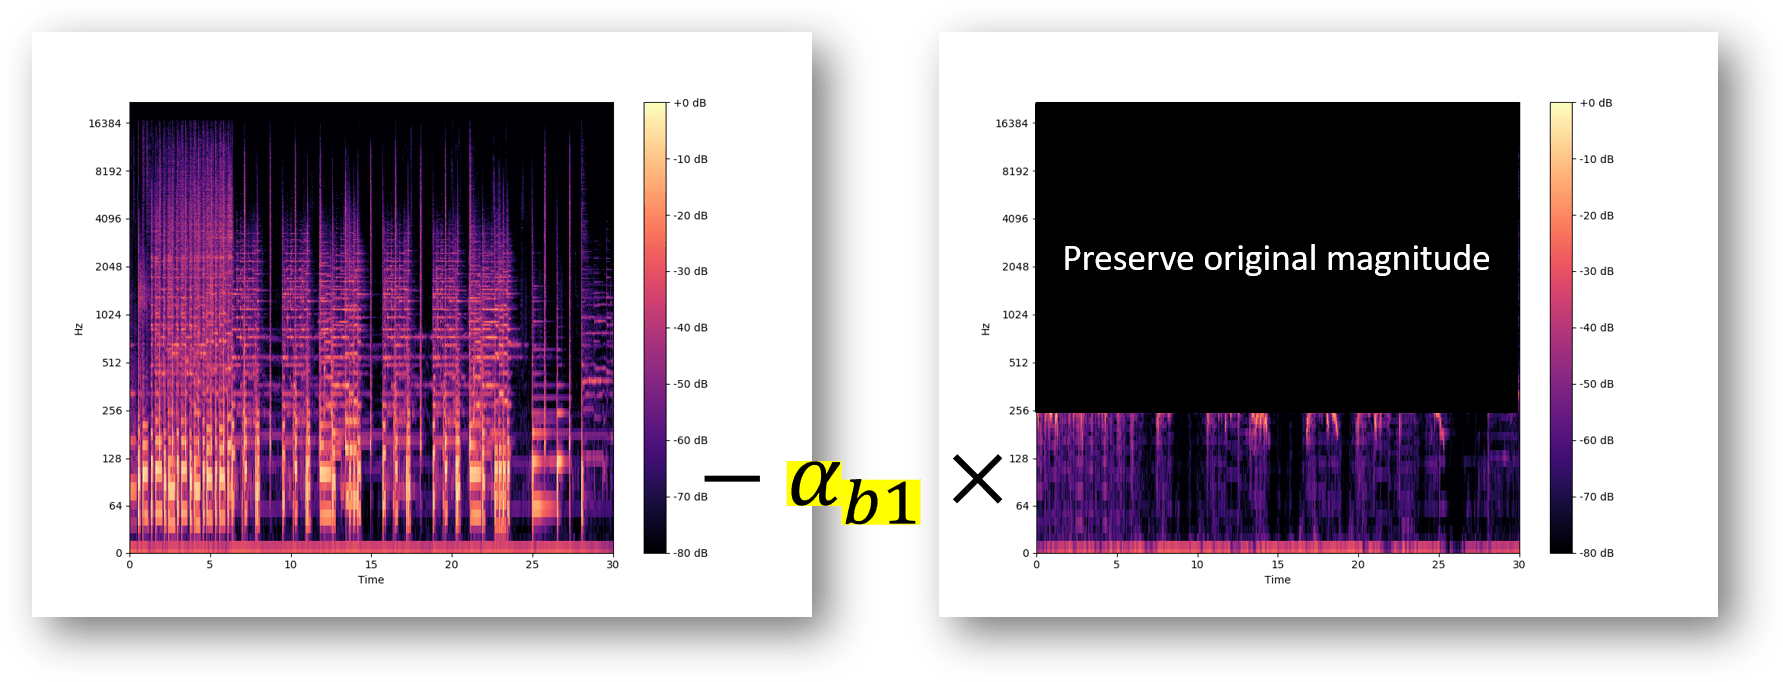
\includegraphics[width=\textwidth]{./figures/chapter04_experiment/Local_Bands_Optimal1.png}
        \caption {Local bands optimal}
        \label{Bands_Optimum_Ratio}
    \end{minipage}
    \hfil
\end{figure}
\begin{figure}[htbp]
    \hfil
    \begin{minipage}[t]{0.65\textwidth}
        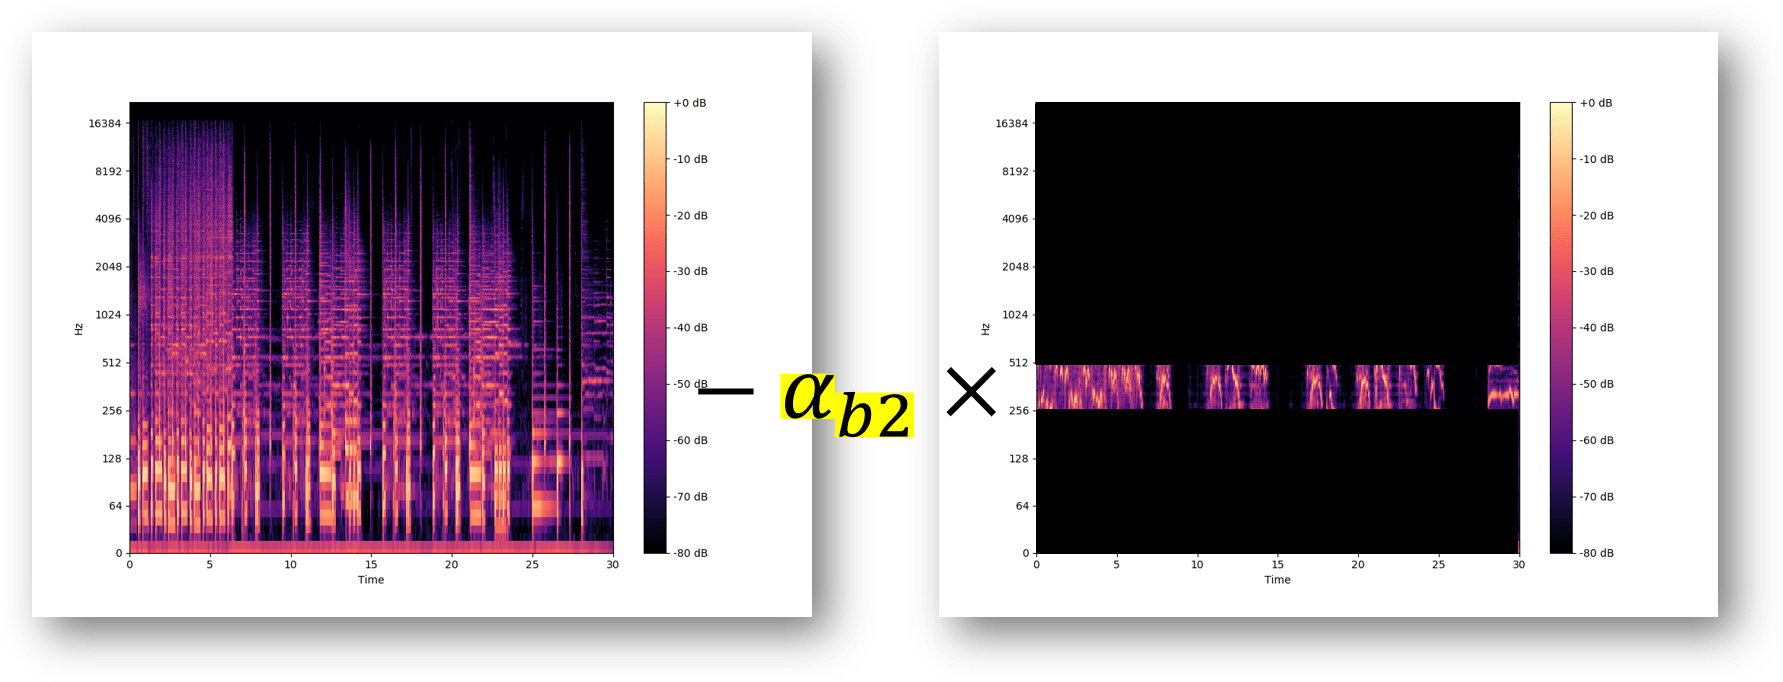
\includegraphics[width=\textwidth]{./figures/chapter04_experiment/Local_Bands_Optimal2.png}
        \caption {Local bands optimal}
        \label{Bands_Optimum_Ratio2}
    \end{minipage}
    \hfil
\end{figure}
\begin{figure}[htbp]
    \hfil
    \begin{minipage}[t]{0.65\textwidth}
        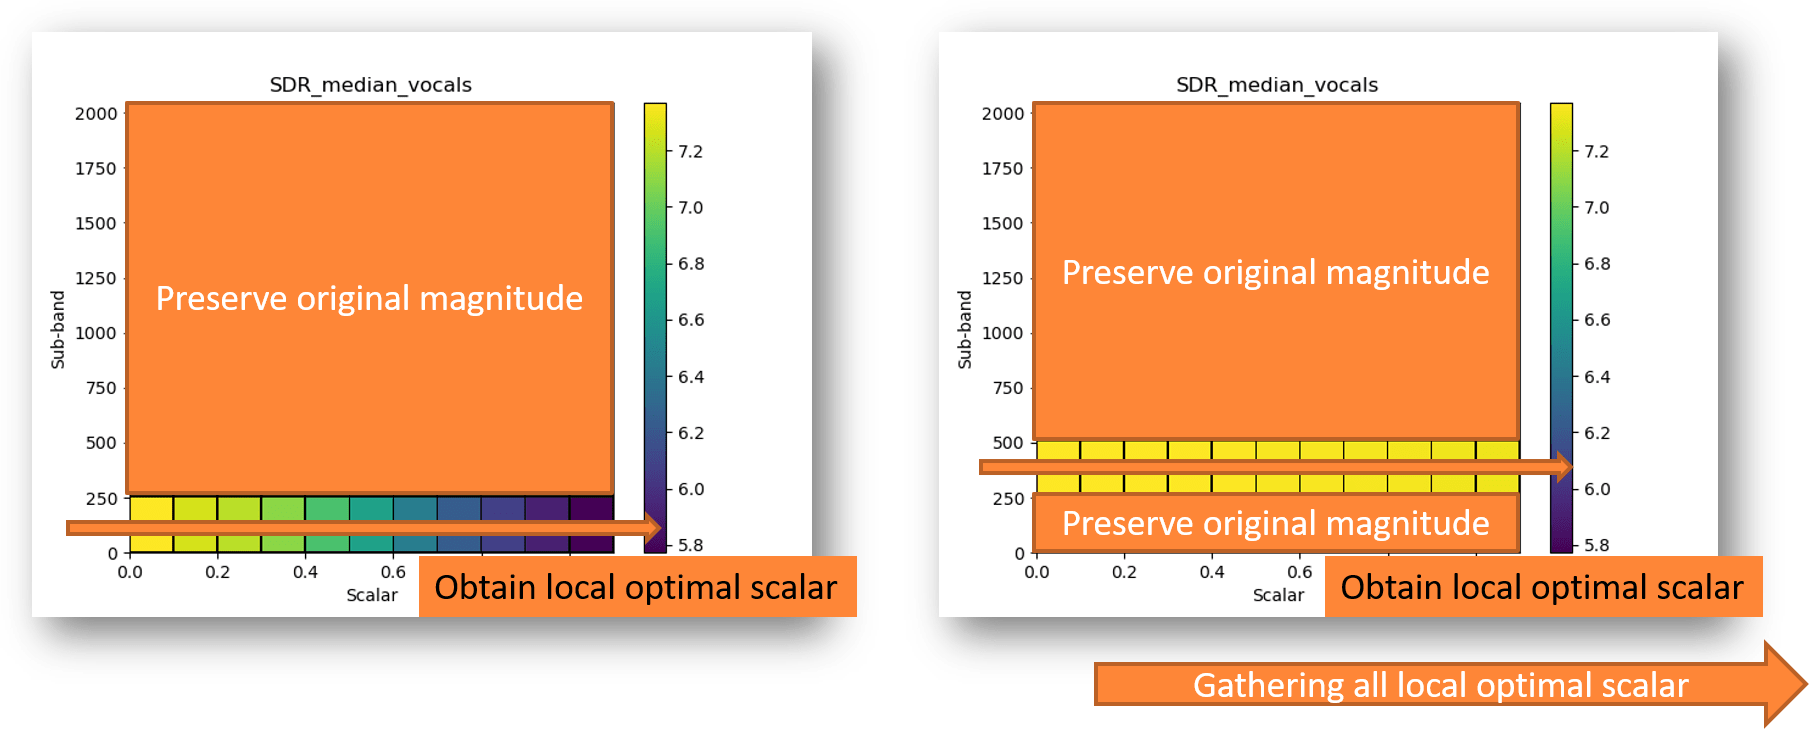
\includegraphics[width=\textwidth]{./figures/chapter04_experiment/Local_Bands_Optimal3.png}
        \caption {Local bands optimal}
        \label{Local_Bands_Optimal3}
    \end{minipage}
    \hfil
\end{figure}

枚舉所有 $\alpha_f$ 難以實現,所以考慮第二種方式,也就是使用簡單的梯度下降架構來訓練,期望每一個 frequency bin (在此研究中總量都為2048個)都能各自算出最好的 $\alpha_f$,改善第一種方式的問題,這邊主要使用最簡單的手法訓練,環繞在一個提出的主架構上(圖\ref{spectrogram_subtraction_NNmethod1}),所有調整架構的實驗中,該架構表現最為出色,其餘架構只以表\ref{spectrogram_subtraction_NNmethod} 呈現,主要討論此方法與第一種方法的差異,而非討論中間梯度下降架構的調整,最終的效果會在下章仔細的探討與分析。梯度下降架構的訓練只在 Musdb18 的訓練集上(共100首),測試集在 Musdb18 的測試集上(共50首),其聲音訊號經由 STFT ,取其 2048 個 frequency bin (F) 與 216 個 frame(T),最後評估的指標使用 Museval。

\begin{table}[htbp]
\centering
\resizebox{\linewidth}{!}{
\begin{tabular}{|c|c|l|l|l|l|l|}
\hline
Magnitude size & 1 layer in neural net & ReLU & Loss function & Batch & Epoch & Optim. method \\ \hline
 & $1\times 2048$ & No & L1Loss & 8 & 200 & ADAM \\ \cline{3-7} 
 & $C\times F$ & No & SmoothL1Loss & 8 & 200 & ADAM \\ \cline{3-7} 
$1\times 2048 \times 512$ & Only apply on stem$_j$ & Yes & L1Loss & 8 & 200 & ADAM \\ \cline{2-7} 
$C\times F\times T$ & $1\times 2048$ & Yes & SmoothL1Loss & 8 & 200 & ADAM \\ \cline{3-7} 
 & $C\times F$ & No & L1Loss & 8 & 200 & ADAM \\ \cline{3-7} 
 & Apply on each stem & No & SmoothL1Loss & 8 & 200 & ADAM \\ \hline
\end{tabular}
}
\caption{過程中梯度下降架構的調整}
\label{spectrogram_subtraction_NNmethod}
\end{table}

\begin{figure}[htbp]
    \hfil
    \begin{minipage}[t]{0.45\textwidth}
        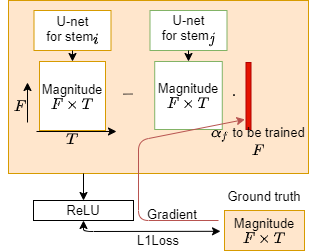
\includegraphics[width=\textwidth]{./figures/chapter04_experiment/spectrogram_subtraction_gradientdecent_method.png}
        \caption {提出的梯度下降架構用以訓練頻譜刪減之對應 $\alpha_f$}
        \label{spectrogram_subtraction_NNmethod1}
    \end{minipage}
    \hfil
\end{figure}

\subsection{注意力模型實驗}
基於 Demucs~\cite{defossez2019music} 與 MMDenseLSTM~\cite{takahashi2018mmdenselstm} 在歌聲分離領域的出眾表現,除了皆以 U-Net 為雛形做衍伸之外,其模型都有個共通點,都使用到了 LSTM~\cite{gers1999learning} 架構,這邊要先稍微提及,此架構起初用在處理長時間序列,可讓深度神經模型觀察到前後文的重複性,透過加入遺忘閥,在遇到長時間輸入訊號時,依舊有不錯的學習效果,但是由於模型結構複雜,因此需要花費較長的時間。歌聲分離領域裡,需要「快」與「準」,除了要準確的預測輸出的音樂訊號,還要夠快,既有的 U-Net 模型預測已經需要不少的時間,如何在觀察前後文的重複性,又要讓模型預測時間不會因此拉長是值得探討的,此時 Google 團隊錄取 2017NIPS\footnote{\url{https://nips.cc/Conferences/2017/Videos}} 的論文「Attention is all you need」~\cite{vaswani2017attention} ,其架構拋棄 RNN 的架構取而代之的是 self-attention 的注意力機制,可以在翻譯領域上有很好的效果,但不導致架構的預測速度。
% file:///C:/Users/hp/Documents/MIR_Lab/report/2Sep2020_report/2Sep2020_report.pdf

% [attention - transformer]
% https://cyeninesky3.medium.com/attention-is-all-you-need-%E5%9F%BA%E6%96%BC%E6%B3%A8%E6%84%8F%E5%8A%9B%E6%A9%9F%E5%88%B6%E7%9A%84%E6%A9%9F%E5%99%A8%E7%BF%BB%E8%AD%AF%E6%A8%A1%E5%9E%8B-dcc12d251449

\subsubsection{Self-attention 架構實驗}
探討在既有的 U-Net 架構~\cite{ronneberger2015u}(圖\ref{Unet_sovia_sattn1}),與 Liu~\cite{liu2020voice} 基於 Dense-UNet~\cite{stoller2018adversarial} 加上 self-attention 架構(圖\ref{Unet_sovia_sattn2})的差異,在下一章可經由實驗結果做比對。
\begin{figure}[htbp]
    \hfil
    \begin{minipage}[t]{0.45\textwidth}
        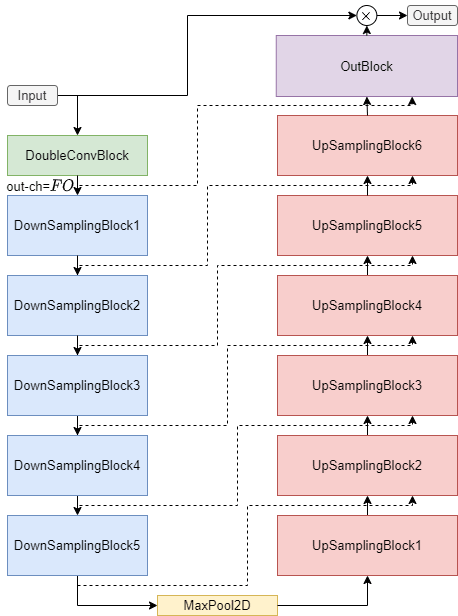
\includegraphics[width=\textwidth]{./figures/chapter04_experiment/Unet_sovia_sattn1.png}
        \caption {既有 U-Net 架構}
        \label{Unet_sovia_sattn1}
    \end{minipage}
    \hfil
\end{figure}
\begin{figure}[htbp]
    \hfil
    \begin{minipage}[t]{0.55\textwidth}
        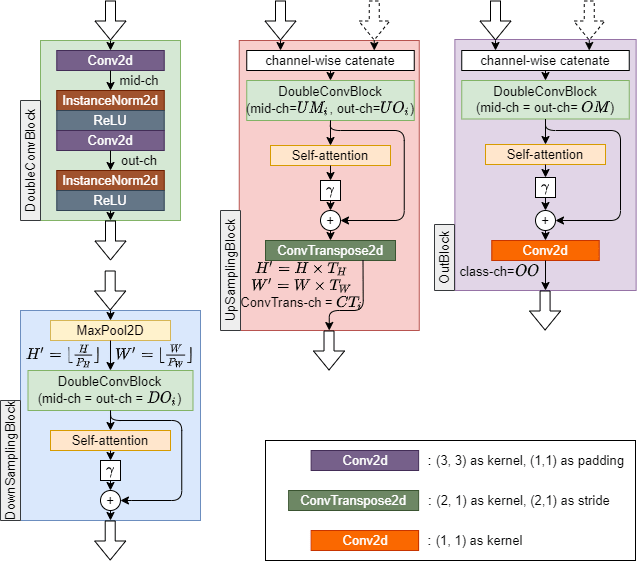
\includegraphics[width=\textwidth]{./figures/chapter04_experiment/Unet_sovia_sattn2.png}
        \caption {對應各子架構}
        \label{Unet_sovia_sattn2}
    \end{minipage}
    \hfil
\end{figure}

適配 self-attention 架構於既有 U-Net 上,做了些許與原文的差異化,本論文將原論文的 $C'$ 設定為 $\left \lfloor C/8 \right \rfloor$而非原文設定的 $C':=5$。另外,U-Net 的 encoder 與 decoder 詳細見下表\ref{UNet_sovia_setting}。

\begin{table}[htbp]
\centering
\begin{tabular}{ccccccc}
\multicolumn{1}{c|}{$i$} & 1 & 2 & 3 & 4 & 5 & 6 \\ \hline
\multicolumn{1}{c|}{$DO_i$} & 32 & 64 & 128 & 256 & 512 &  \\
\multicolumn{1}{c|}{$UM_i$} & 1024 & 512 & 256 & 128 & 64 & 32 \\
\multicolumn{1}{c|}{$UO_i$} & 512 & 256 & 128 & 64 & 32 & 16 \\ \hline
\multicolumn{1}{l}{$FO$=1} & \multicolumn{1}{l}{$OM$=16} & \multicolumn{1}{l}{$OO$=1} & \multicolumn{1}{l}{$P_H$=2} & \multicolumn{1}{l}{$P_W$=1} & \multicolumn{1}{l}{$T_H$=2} & \multicolumn{1}{l}{$T_W$=1}
\end{tabular}
\caption{U-Net6 (baseline) 參數表}
\label{UNet_sovia_setting}
\end{table}

\subsubsection{Attention Gate 架構實驗}
本論文主要探討在既有的 U-Net 架構~\cite{ronneberger2015u}(圖\ref{Unet_sovia_sattn1}),再參考 oktay~\cite{oktay2018attention} 等人提出的 attention U-Net 架構(圖\ref{Unet_sovia_AG1}與圖\ref{Unet_sovia_AG2}),改進既有的 U-Net ,並討論其差異,在下一章可經由實驗結果做比對。可以注意的是圖\ref{attention_gate1} 上的最後有一個調控的 $\alpha$ 參數,為求實驗方便在此固定為 $\alpha:=1$,未來可實驗讓機器自我訓練出該參數的值。

\begin{figure}[htbp]
    \hfil
    \begin{minipage}[t]{0.3\textwidth}
        \centering
        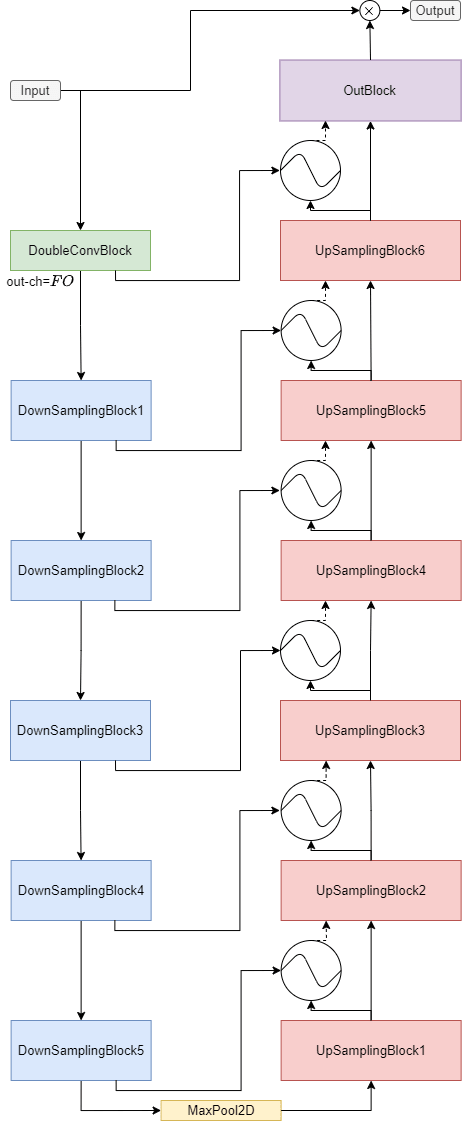
\includegraphics[width=\textwidth]{./figures/chapter04_experiment/Unet_sovia_AG1.png}
        \caption {加上 attention gate 的 U-Net 架構}
        \label{Unet_sovia_AG1}
    \end{minipage}
    \begin{minipage}[t]{0.65\textwidth}
        \centering
        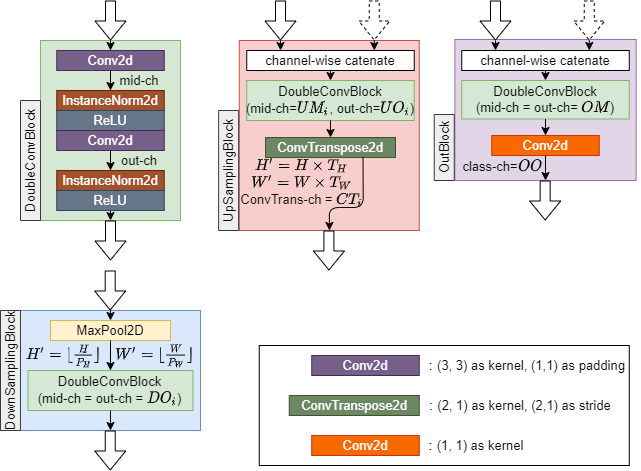
\includegraphics[width=\textwidth]{./figures/chapter04_experiment/Unet_sovia_AG2.png}
        \caption {對應各子架構}
        \label{Unet_sovia_AG2}
    \end{minipage}
    \hfil
\end{figure}

\subsection{模型剪枝實驗}
本論文基於深度可分卷積與 Inverted Residuals 套用在既有 U-Net,前者可以大幅減少模型參數伴隨較大的效能損失,架構細節如圖\ref{MobileUnetV1_1} 與圖\ref{MobileUnetV1_2} ;後者便是稍微對前者方法提升計算量伴隨效果提升,架構細節如圖\ref{MobileUnetV2_1} 與圖\ref{MobileUnetV2_2} 。實際實驗結果在下章討論。

\begin{figure}[htbp]
    \hfil
    \begin{minipage}[t]{0.3\textwidth}
        \centering
        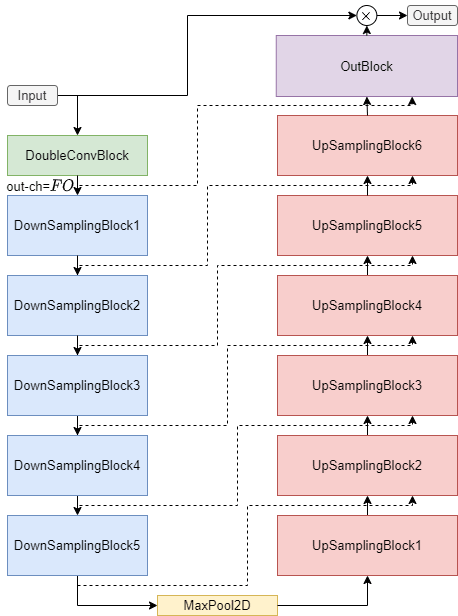
\includegraphics[width=\textwidth]{./figures/chapter04_experiment/MobileUnetV1_1.png}
        \caption {加上深度可分卷積的 U-Net 架構}
        \label{MobileUnetV1_1}
    \end{minipage}
    \begin{minipage}[t]{0.65\textwidth}
        \centering
        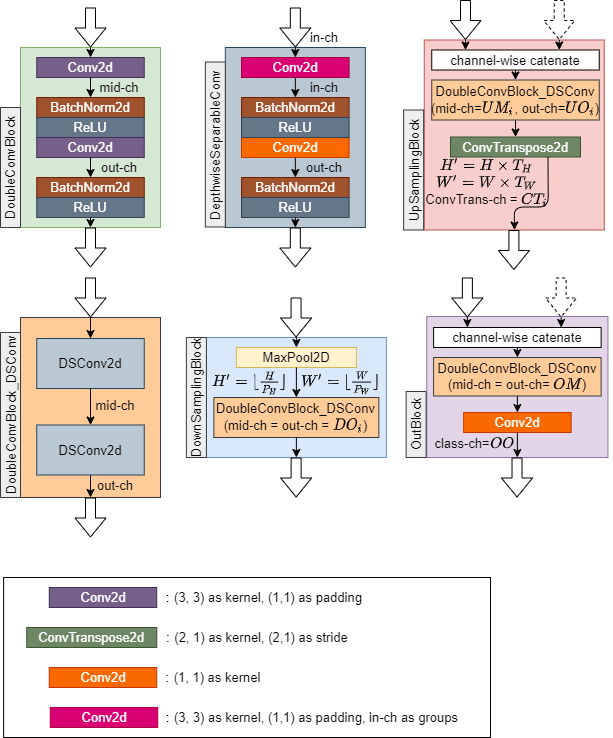
\includegraphics[width=\textwidth]{./figures/chapter04_experiment/MobileUnetV1_2.png}
        \caption {對應各子架構}
        \label{MobileUnetV1_2}
    \end{minipage}
    \hfil
\end{figure}

\begin{figure}[htbp]
    \hfil
    \begin{minipage}[t]{0.3\textwidth}
        \centering
        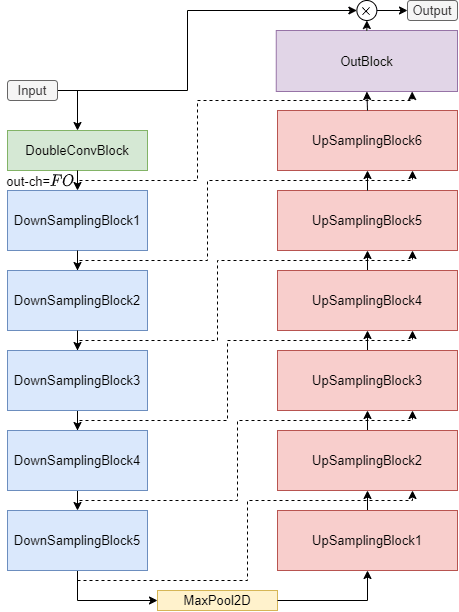
\includegraphics[width=\textwidth]{./figures/chapter04_experiment/MobileUnetV2_1.png}
        \caption {加上 inverted residual block 的 U-Net 架構}
        \label{MobileUnetV2_1}
    \end{minipage}
    \begin{minipage}[t]{0.6\textwidth}
        \centering
        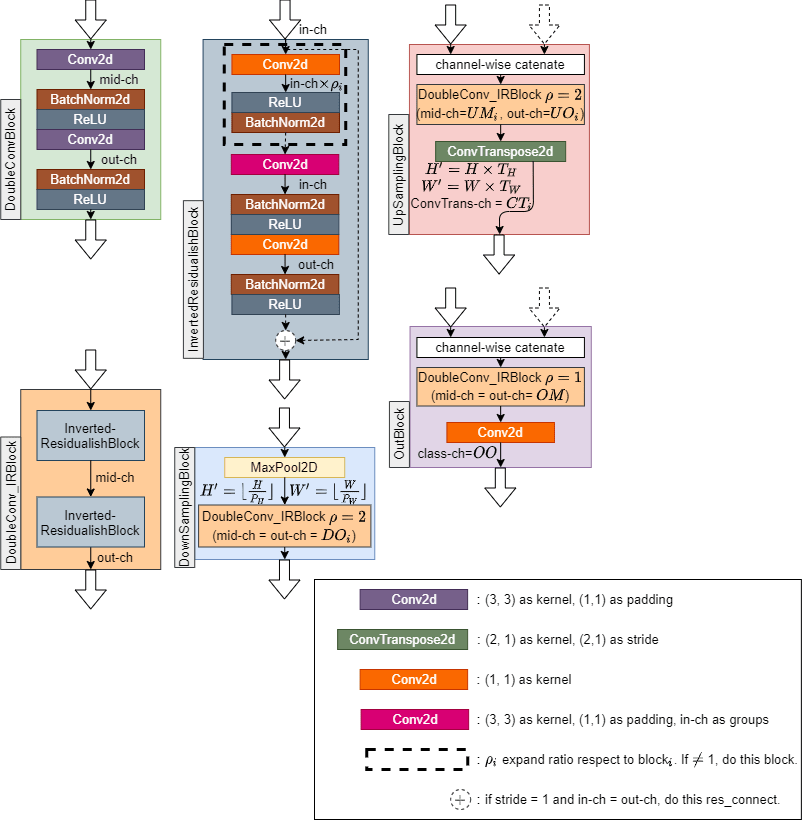
\includegraphics[width=\textwidth]{./figures/chapter04_experiment/MobileUnetV2_2.png}
        \caption {對應各子架構}
        \label{MobileUnetV2_2}
    \end{minipage}
    \hfil
\end{figure}

\clearpage

\subsection{模型量化實驗}
本論文中,主要使用 FaceBook 所提出的 QNNPACK~\cite{dukhan2018qnnpack} 對既有 U-Net 做量化至 int8,值得注意的是,在量化之前,依照常規的手法,會先對模型做融合的操作\footnote{\url{https://pytorch.org/tutorials/recipes/recipes/dynamic_quantization.html}},主要是讓機器在計算 biases 與 ReLU 可以更加快速,其主要的融合方法見圖\ref{quantization2}。

\begin{figure}[htbp]
    \hfil
    \begin{minipage}[t]{1.0\textwidth}
        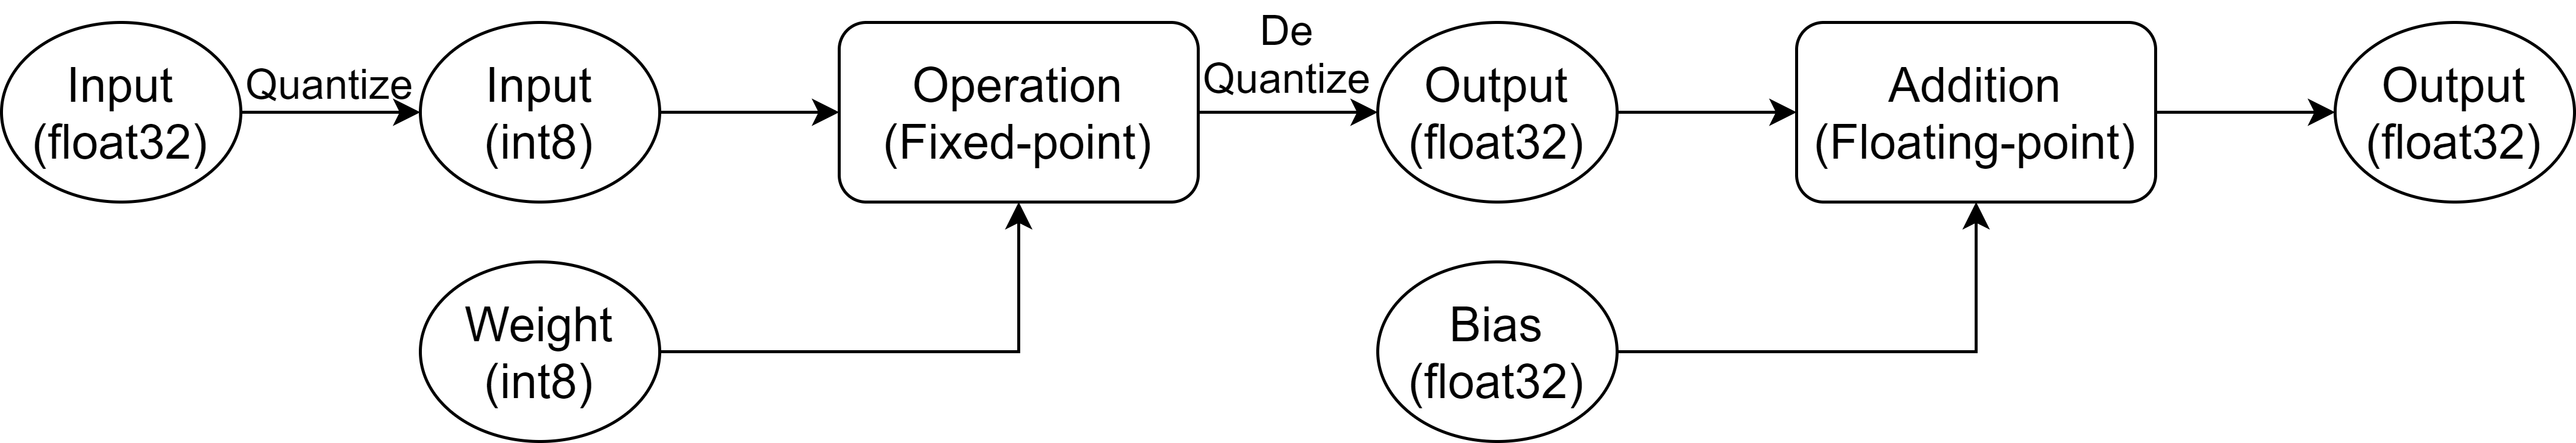
\includegraphics[width=\textwidth]{./figures/chapter04_experiment/quantization2.png}
        \caption {量化過程圖}
        \label{quantization2}
    \end{minipage}
    \hfil
\end{figure}